\section{Processi di supporto}
    \subsection{Documentazione}
        \subsubsection{Scopo}
        Lo scopo del processo di documentazione è di redigere e mantenere la documentazione durante l'intero \glo{Ciclo di vita}{ciclo di vita} del software. La corretta implementazione del processo deve:
        \begin{itemize}
            \item dare una chiara visione dei documenti che devono essere prodotti durante il \glo{Ciclo di vita}{ciclo di vita} del software;
            \item fornire le norme necessarie alla stesura dei documenti;
            \item produrre documenti formali coerenti.
        \end{itemize}
        \subsubsection{Template}
        È stato creato un template \LaTeX{} per garantire che tutti i documenti creati dal \glo{Gruppo}{gruppo} abbiamo la stessa struttura grafica e lo stesso stile di formattazione. Ogni membro del \glo{Gruppo}{gruppo} deve creare i documenti richiesti utilizzando tale template e deve ridurre al minimo indispensabile eventuali variazioni personali nella formattazione.
        \subsubsection{Struttura dei documenti}
                \paragraph{Prima pagina}
                La prima pagina di ogni documento deve presentare la seguente struttura:
                \begin{itemize}
                    \item logo del \glo{Gruppo}{gruppo};
                    \item titolo del documento;
                    \item informazioni del documento:
                    \begin{itemize}
                        \item versione;
                        \item data di creazione;
                        \item data di ultima modifica;
                        \item stato del documento;
                        \item redattori del documento;
                        \item verificatori;
                        \item responsabile approvazione;
                        \item lista di distribuzione;
                        \item email del \glo{Gruppo}{gruppo}.
                    \end{itemize}
                \end{itemize}
                \paragraph{Registro delle modifiche}
                La seconda pagina di ogni documento formale deve contenere una tabella con la lista delle modifiche apportate al documento. Ogni riga della tabella deve essere compilata per intero con le seguenti informazioni:
                \begin{itemize}
                    \item versione del documento successiva alla modifica;
                    \item data in cui è stata eseguita la modifica;
                    \item autore della modifica;
                    \item ruolo dell'autore;
                    \item descrizione concisa della modifica apportata.
                \end{itemize}
                \paragraph{Indice}
                Nella pagina successiva alla fine del registro delle modifiche ogni documento formale deve contenere l'indice dei suoi contenuti; tale indice deve permettere la lettura \glo{Ipertestuale}{ipertestuale} del documento. L'indice deve essere numerato a partire da 1, ogni sottosezione riparte da 1 e aggiunge il proprio indice a quello del padre separandolo con un punto. Eventuali appendici invece di essere numerate saranno indicate con lettere maiuscole a partire da A seguendo l'ordine alfabetico internazionale.
                \paragraph{Note a piè di pagina}
                Eventuali note vanno indicate in basso a sinistra nella pagina in cui compaiono con il loro numero identificativo e la loro descrizione.
                \paragraph{Contenuto principale}
                Tutte le pagine successive all'indice del documento devono contenere un'intestazione e un piè di pagina.
                L'intestazione deve contenere:
                \begin{itemize}
                    \item nome della sezione allineato a sinistra;
                    \item nome del documento allineato a destra.
                \end{itemize}
                Il piè di pagina deve contenere:
                \begin{itemize}
                    \item nome del \glo{Gruppo}{gruppo} e del progetto allineati a sinistra;
                    \item pagina corrente rispetto alle pagine totali del documento allineate a destra.
                \end{itemize}
        \subsubsection{Norme tipografiche}
                \paragraph{Glossario}
                Ogni parola contenuta nel \gl{} deve essere scritta in corsivo e contrassegnata da una "G" a pedice come da esempio:\\
                \centerline{\textit{termine\textsubscript{G}}}
                \paragraph{Stile del testo}
                Per una facilitare la stesura del documento, migliorarne correttezza e leggibilità, TexStudio mette a disposizione dei tool per il controllo grammaticale. Ogni membro del \glo{Gruppo}{gruppo} deve controllare nelle impostazioni del proprio strumento che siano attivati:
                \begin{itemize}
                	\item \textbf{individua ripetizioni:} durante la scrittura del documento, se una parola viene ripetuta troppo viene sottolineata di verde;
                	\item \textbf{individua errori ortografici:} gli errori vengono sottolineati di rosso;
                	\item \textbf{lingua predefinita:} italiano.
                \end{itemize}
                Le seguenti convenzioni devono essere rispettate nella stesura dei documenti:
                \begin{itemize}
                    \item \textbf{grassetto:} deve essere utilizzato nei seguenti casi:
                        \begin{itemize}
                            \item titoli di sezioni e paragrafi;
                            \item termini di elenchi puntati per i quali si fornisce una descrizione;
                            \item riferimenti alle revisioni di avanzamento.
                        \end{itemize}
                    \item \textbf{corsivo:} deve essere utilizzato nei seguenti casi:
                        \begin{itemize}
                            \item nome del \glo{Gruppo}{gruppo};
                            \item nome del proponente;
                            \item nome del progetto;
                            \item citazioni;
                            \item abbreviazioni;
                            \item parole presenti nel glossario;
                            \item ruoli del progetto;
                            \item nomi dei documenti.
                        \end{itemize}
                    \item \textbf{monospace:} deve essere utilizzato nei seguenti casi:
                        \begin{itemize}
                            \item nomi di file;
                            \item codice di programmazione;
                            \item indirizzi email.
                        \end{itemize}
                    \item \textbf{maiuscolo:} le uniche parole che possono essere scritte interamente a caratteri maiuscoli sono gli acronimi e le sigle.
                \end{itemize}
                \paragraph{Titoli}
                I titoli delle sezioni e dei paragrafi vanno scritti con solo la prima lettera maiuscola a meno di nomi propri e di termini indicati nella sezione \ref{sec:formati}.
                \paragraph{Elenchi puntati}
                Le seguenti convenzioni devono essere rispettate nella creazione di elenchi puntati:
                \begin{itemize}
                    \item ogni elemento dell'elenco deve iniziare con la lettera minuscola a meno che non sia un nome proprio;
                    \item ogni elemento dell'elenco tranne l'ultimo deve terminare con un punto e virgola;
                    \item l'ultimo elemento dell'elenco deve terminare con il punto.
                \end{itemize}
                \paragraph{Formati}\label{sec:formati}
                I seguenti formalismi devono essere utilizzati durante la stesura dei documenti:
                \begin{itemize}
                    \item \textbf{date:} le date presenti nei documenti devono seguire lo standard \glo{ISO}{ISO} 8601:2004 (vedi riferimento \ref{sec:iso8601}):\\\\
                    \centerline{YYYY-MM-GG}\\
                    dove:
                    \begin{itemize}
                        \item \textbf{YYYY:} rappresenta l'anno espresso con quattro cifre;
                        \item \textbf{MM:} rappresenta il mese espresso con due cifre;
                        \item \textbf{GG:} rappresenta il giorno espresso con due cifre.
                    \end{itemize}
                    È possibile utilizzare il comando \LaTeX{} \texttt{\textbackslash frmdata\{GG\}\{MM\}\{YYYY\}} per la formattazione delle date.
                    \item \textbf{orari:} gli orari presenti nei documenti devono seguire lo standard \glo{ISO}{ISO} 8601:2004 (vedi riferimento \ref{sec:iso8601}):\\\\
                    \centerline{hh:mm}\\
                    dove:
                    \begin{itemize}
                        \item \textbf{hh:} rappresentano le ore espresse con due cifre da 00 a 23;
                        \item \textbf{mm:} rappresentano i minuti espressi con due cifre da 00 a 59.
                    \end{itemize}
                    È possibile utilizzare il comando \LaTeX{} \texttt{\textbackslash frmora\{hh\}\{mm\}} per la formattazione delle ore.
                    \item \textbf{valute:} le valute presenti nei documenti devono essere scritte utilizzando il simbolo della valuta usata seguito dal numero. Le cifre decimali devono essere separate dalla virgola, le cifre non decimali devono essere separate da un punto a gruppi di tre:
                    \centerline{[Simbolo valuta] 1.234.567,89}
                    Ad esempio: € 3.869,25
                    \item \textbf{nomi ricorrenti:}
                    I seguenti termini ricorrenti vanno sempre inseriti con i relativi comandi \LaTeX{} forniti dal template per garantire omogeneità in tutti i documenti:
                    \begin{itemize}
                        \item nome del \glo{Gruppo}{gruppo};
                        \item email di riferimento del \glo{Gruppo}{gruppo};
                        \item nome del proponente;
                        \item nome del progetto svolto;
                        \item ruoli di progetto;
                        \item nomi dei documenti senza versione;
                        \item nomi dei documenti con versione;
                        \item revisioni di avanzamento del progetto.
                    \end{itemize}
                \end{itemize}
                \paragraph{Nomi propri}
                    I nomi propri di persona devono essere scritti come nome e cognome.
        \subsubsection{Componenti grafiche}
                \paragraph{Tabelle}
                Tutte le tabelle devono avere un indice numerico univoco che le identifichi all'interno del documento ed una breve didascalia. Le tabelle devono essere centrate orizzontalmente.
                \paragraph{Immagini}
                Tutte le immagini inserite all'interno di un documento devono avere ampi margini orizzontali che le separino in modo netto dai paragrafi precedenti e successivi per migliorare la leggibilità. Le immagini devono essere centrate orizzontalmente e devono avere larghezza fissa. I diagrammi \glo{UML}{UML} devono essere inseriti nei documenti come immagini.
        \subsubsection{Classificazione dei documenti}\label{sec:classificazionedocumenti}
            \paragraph{Documenti informali}
            Tutti i documenti non ancora approvati dal responsabile di progetto sono da ritenersi informali e pertanto ad uso unicamente interno.
            \paragraph{Documenti formali}
            Un documento diventa formale in seguito all'approvazione da parte del \responsabilediprogetto. Solo i documenti formali possono essere distribuiti all'esterno del \glo{Gruppo}{gruppo}. Prima di poter essere approvato un documento deve essere verificato come descritto nella sezione \ref{sec:ciclodivitadoc} e secondo le procedure descritte nella sezione \ref{sec:verifica}.
            \paragraph{Verbali}\label{sec:verbali}
            Per ogni incontro deve essere nominato un segretario che si occuperà della stesura di un verbale. Il verbale deve contenere i seguenti punti:
            \begin{itemize}
                \item \textbf{estremi della riunione:}
                    \begin{itemize}
                        \item data;
                        \item ora inizio;
                        \item ora fine;
                        \item luogo dove si è svolto l'incontro;
                        \item lista dei partecipanti;
                        \item lista degli assenti con eventuali motivazioni;
                        \item nome del segretario.
                    \end{itemize}
                \item \textbf{ordine del giorno:} elenco degli argomenti che saranno discussi;
                \item \textbf{corpo del verbale:} verbale dell'incontro;
                \item \textbf{decisioni prese:} elenco delle decisioni prese identificate in modo univoco.
            \end{itemize}
            Una volta approvato dal \responsabilediprogetto{} il verbale deve essere distribuito a tutti i componenti del \glo{Gruppo}{gruppo}, nel caso di verbale esterno dovrà essere inviato anche al proponente.
            I nomi dei file dei verbali devono rispettare il seguente formato:\\\\
            \centerline{\texttt{Verbale[Tipologia]\_[ID]\_[Data riunione].pdf}}\\
            dove:
            \begin{itemize}
                \item \textbf{tipologia:} \texttt{Esterno} o \texttt{Interno};
                \item \textbf{ID:} identificativo numerico, si distingue tra verbali interni ed esterni, parte da 1;
                \item \textbf{data riunione:} data in cui si è svolta la riunione in formato YYYYMMGG.
            \end{itemize}
	        I nomi delle decisioni devono rispettare il seguente formato:\\\\
            \centerline{\texttt{V[ID tipologia]\_[ID].[Numero decisione]}}\\
            dove:
            \begin{itemize}
            	\item \textbf{ID Tipologia:} \texttt{I} o \texttt{E} che significano rispettivamente Interno o Esterno;
            	 \item \textbf{ID:} identificativo numerico, si distingue tra verbali interni ed esterni, parte da 1;
            	 \item \textbf{Numero decisione:} numero crescente univoco per quantificare la decisione.
            \end{itemize}
			Per la redazione dell'elenco delle decisioni è necessario utilizzare i comandi \LaTeX
			\begin{itemize}
				\item \texttt{\textbackslash itemVE} - per i verbali esterni;
				\item \texttt{\textbackslash itemVI}  - per quelli interni.
			\end{itemize}
            \paragraph{Versionamento}\label{sec:versionamento}
            Tutti i documenti formali ed informali devono essere identificati da una versione, ad ogni nuova versione deve corrispondere una riga nel registro delle modifiche.
            La versione corrente di un documento deve sempre essere riportata all'interno del documento stesso e va inoltre indicata in coda al nome del file con il seguente formato:\\\\
            \centerline{\texttt{NomeDocumento\_vX.Y.Z.pdf}}\\
            dove:
            \begin{itemize}
                \item \textbf{X:}
                \begin{itemize}
                    \item inizia da 0;
                    \item viene incrementato solo dal \responsabilediprogetto{} all'approvazione del documento;
                    \item non può essere maggiore del numero di revisioni.
                \end{itemize}
                \item \textbf{Y:}
                \begin{itemize}
                    \item inizia da 0;
                    \item viene incrementato solo dai \verificatori{} ad ogni verifica eseguita;
                    \item quando viene incrementato X, viene riportato a 0.
                \end{itemize}
                \item \textbf{Z:}
                \begin{itemize}
                    \item inizia da 0;
                    \item viene incrementato solo dai redattori al completamento di ogni task di modifica del documento;
                    \item quando vengono incrementati X o Y, viene riportato a 0.
                \end{itemize}
            \end{itemize}
        \subsubsection{Procedure}
            \paragraph{Creazione di un documento}
            Viene fornito nel \glo{Repository}{repository} un file \LaTeX{} generico denominato \texttt{templateDoc.tex} che contiene il template da utilizzare. Per creare un nuovo documento è sufficiente copiare il file ed inserire il contenuto necessario. Ogni redattore è tenuto a scaricare e mantenere aggiornati tutti i file necessari al template presenti nel \glo{Repository}{repository}.
            \paragraph{Ciclo di vita dei documenti}\label{sec:ciclodivitadoc}
            Tutti i documenti tranne i verbali devono seguire il \glo{Ciclo di vita}{ciclo di vita} descritto di seguito (vedi anche figura \ref{fig:ciclovitadoc}):
            \begin{enumerate}
                \item al termine della stesura di un documento, i redattori ne richiedono la verifica al \responsabile;
                \item il \responsabile{} assegna la verifica ad un \verificatore;
                \item il \verificatore{} segnala eventuali modifiche o correzioni da eseguire ai redattori;
                \item quando il \verificatore{} ritiene che il documento sia pronto per l'approvazione la richiede al \responsabile;
                \item il \responsabile{} approva il documento rendendolo formale o lo rifiuta fornendo le motivazioni.
            \end{enumerate}
            \begin{figure}[h]
		        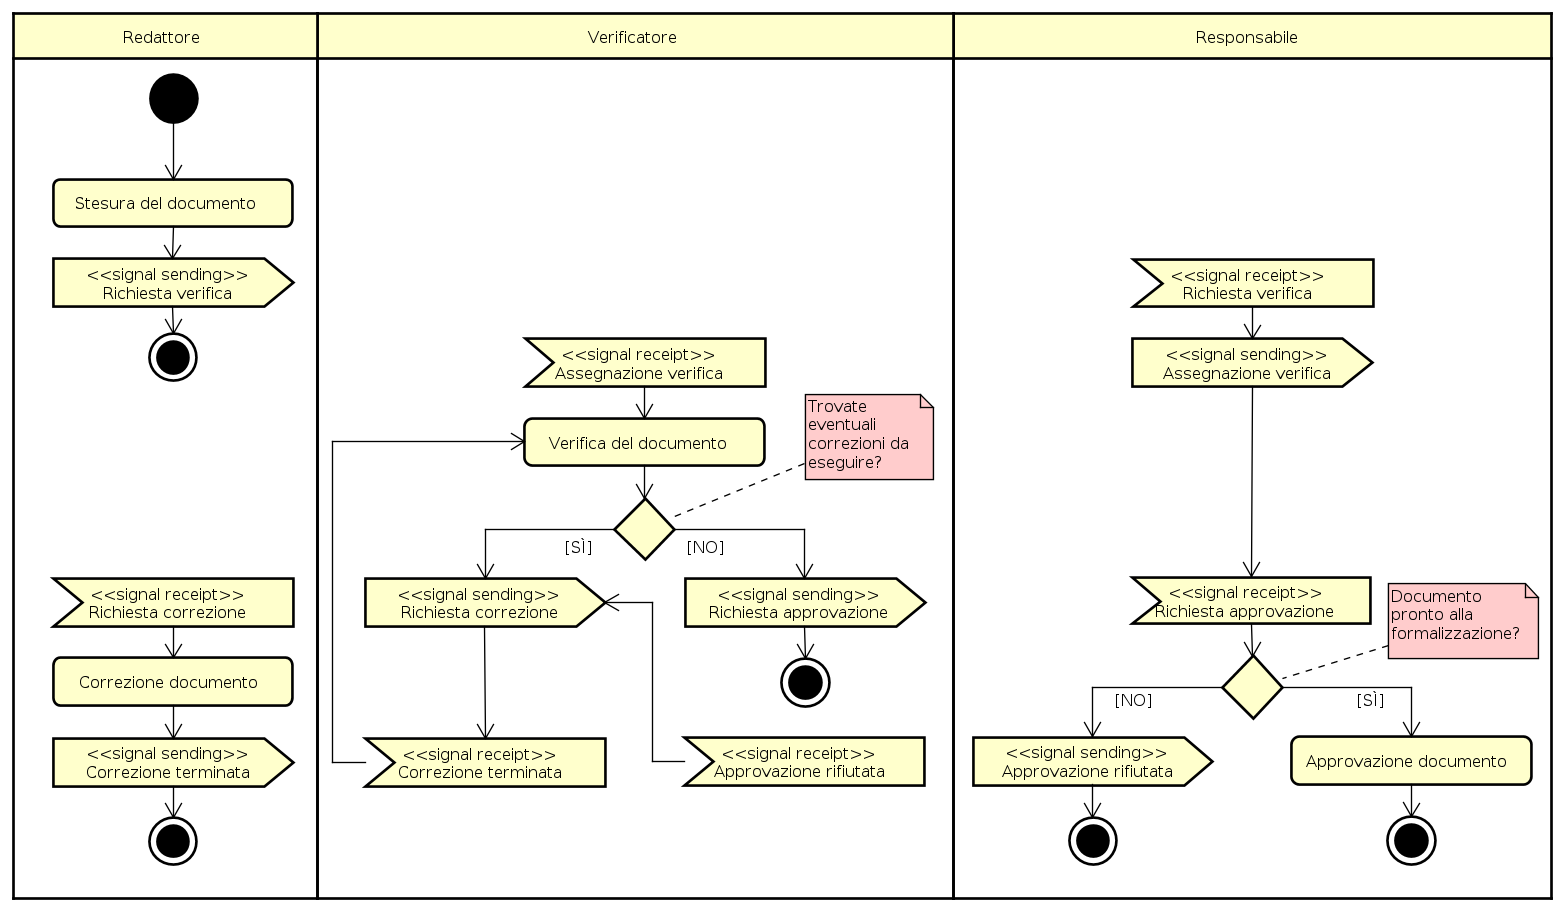
\includegraphics[width=\textwidth]{img/ciclo_di_vita_doc}
		        \captionof{figure}{\glo{Ciclo di vita}{Ciclo di vita} di un documento. Riferita nella sezione \ref{sec:ciclodivitadoc}}
                \label{fig:ciclovitadoc}
	        \end{figure}\mbox{}\\
        \subsubsection{Strumenti}
            \paragraph{Latex}
            Per la stesura dei documenti è stato scelto il \glo{Linguaggio di markup}{linguaggio di markup} \LaTeX{}. Questo permette di preparare documenti formali divisi in sezioni facilitando la collaborazione tra più editori, di separare il contenuto dalla formattazione grafica e di gestire in maniera automatica vari elementi del testo.
            % 1)descrizione veloce dell'app
            % 2)cosa ci permette di fare
            % 3) perche l'abbiamo scelta
            % 4) indirizzo dove collegarsi
            \paragraph{TeXstudio}\label{sec:texstudio}
            % 1)descrizione veloce dell'app
            \glo{TeXstudio}{TeXstudio} è un editor per la creazione di documenti in \LaTeX. Questo software offre un ambiente di lavoro completo per aiutare la stesura dei documenti. Inoltre integra un compilatore e visualizzatore PDF per il documento prodotto. Tra le principali funzionalità sono presenti:
            \begin{itemize}
            	\item evidenziazione della sintassi;
            	\item strumenti per il controllo ortografico;
            	\item completamento automatico.
            \end{itemize}
            % 2)cosa ci permette di fare
	        Questo strumento è utilizzato durante le attività di analisi e progettazione per redigere i documenti necessari. La versione in uso è la 2.11.0 o superiore. \\
            % 3) perche l'abbiamo scelta
            Le principali motivazioni che hanno portato il \glo{Gruppo}{gruppo} alla scelta di questo strumento sono:
            \begin{itemize}
            	\item gratuito;
            	\item \glo{Cross-platform}{cross-platform};
            	\item già conosciuto da alcuni membri del \glo{Gruppo}{gruppo}.
	        \end{itemize}
            % 4) indirizzo dove collegarsi
            Indirizzo per il download:
			\begin{center}
	            \url{http://www.texstudio.org}
	        \end{center}

    \subsection{Verifica}\label{sec:verifica}
        \subsubsection{Scopo}
        Lo scopo del processo di verifica è di garantire che ogni attività dei processi svolti non introduca errori nel prodotto e che soddisfi i requisiti o le condizioni necessarie per essere considerata accettabile. La corretta implementazione del processo deve:
        \begin{itemize}
            \item fornire le procedure di verifica necessarie;
            \item individuare i criteri per la verifica;
            \item individuare eventuali difetti perchè possano essere corretti.
        \end{itemize}

        \subsubsection{Procedure}
            \paragraph{Analisi}
                \subparagraph{Analisi statica}
                Tecnica utilizzata per l'analisi e la verifica del codice sorgente e della documentazione associata. Può essere applicata secondo due strategie:
                \begin{itemize}
                    \item \textbf{\glo{Walkthrough}{walkthrough}:} lettura completa del codice sorgente da analizzare. Va utilizzata unicamente durante le prime \glo{Fase}{fasi} del progetto in quanto risulta onerosa e non efficiente. Gli \analisti{} che la utilizzano devono stilare una lista di controllo con gli errori rilevati più frequentemente;
                    \item \textbf{\glo{Inspection}{inspection}:} lettura mirata del codice sorgente da analizzare. È necessario avere una lista di controllo per poter localizzare eventuali punti critici in cui cercare errori. Dopo ogni analisi la lista di controllo deve essere incrementata con eventuali nuovi errori rilevati.
                \end{itemize}
                \subparagraph{Analisi dinamica}
                Tecnica per l'analisi del prodotto software, richiede l'esecuzione del programma e viene eseguita tramite dei test che verificano il funzionamento del prodotto. I test devono essere ripetibili e a parità di condizioni iniziale e ambiente devono fornire lo stesso output. Per ogni test deve quindi essere definito:
                \begin{itemize}
                    \item \textbf{ambiente:} sistema hardware e software in cui viene eseguito il test;
                    \item \textbf{stato iniziale:} stato iniziale da cui si parte ad eseguire il test;
                    \item \textbf{input:} input inserito;
                    \item \textbf{output:} output atteso.
                \end{itemize}
            \paragraph{Task di verifica}\label{sec:taskverifica}
            La gestione dei task di verifica avviene tramite la creazione di ticket nell'applicazione \glo{Teamwork}{Teamwork} che viene descritta nella sezione \ref{sec:teamwork}. Al termine di ogni ticket il \responsabilediprogetto{} dovrà seguire la seguente procedura:
            \begin{enumerate}
                \item creare un ticket di verifica con i riferimenti al task da verificare e contrassegnarlo con la dicitura \cit{[VERIFICA]};
                \item assegnare il ticket creato ad un \verificatore;
                \item al completamento del ticket di verifica contrassegnare il ticket originale con la dicitura \cit{[VERIFICATO]}.
            \end{enumerate}
            Vedi anche figura \ref{fig:verificagestione}.

            \paragraph{Gestione delle anomalie}\label{sec:gestioneanomalie}
            La gestione delle anomalie durante il processo di verifica avviene tramite la creazione di ticket nell'applicazione \glo{Teamwork}{Teamwork} che viene descritta nella sezione \ref{sec:teamwork}. Nel caso in cui un \verificatore{} dovesse trovare delle anomalie durante un task di verifica queste dovranno essere gestite nel seguente modo:
            \begin{enumerate}
                \item deve essere creato un subticket contrassegnato dalla dicitura \cit{[BUG]} per ogni anomalia riscontrata;
                \item assegnare i subticket creati agli assegnatari del task di cui si sta eseguendo la verifica;
                \item al completamento di tutti i subticket chiudere il ticket di verifica.
            \end{enumerate}
            Vedi anche figura \ref{fig:verificagestione}.

            \begin{figure}[h]
		        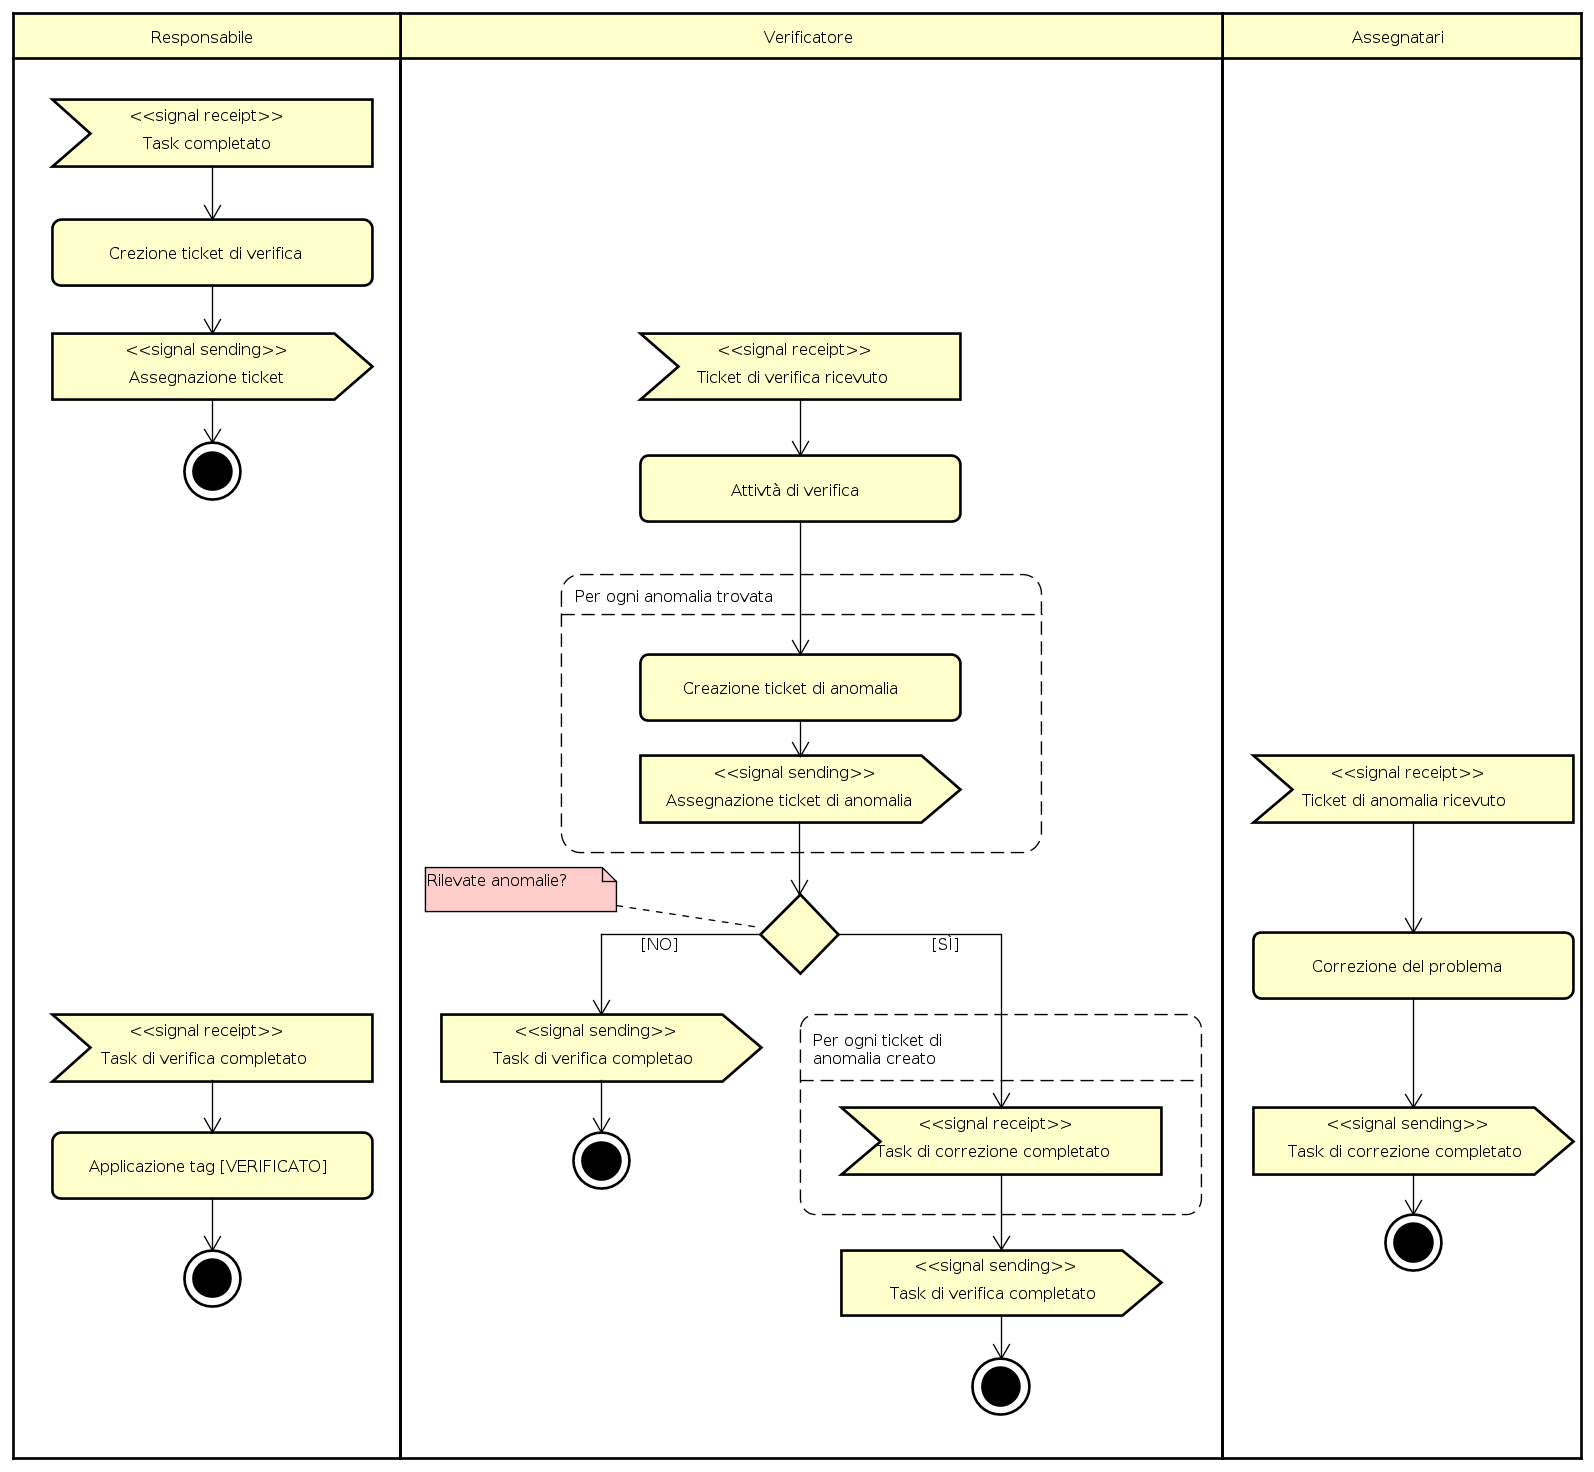
\includegraphics[width=\textwidth]{img/verifica_gestione_task}
		        \captionof{figure}{Procedura di verifica dei task e gestione delle anomalie. Riferita nelle sezioni \ref{sec:taskverifica} e \ref{sec:gestioneanomalie}}
                \label{fig:verificagestione}
	        \end{figure}\mbox{}\\

        \subsubsection{Strumenti}
            \paragraph{Verifica ortografica}
            Viene utilizzato il correttore in tempo reale integrato nell'applicazione \glo{TeXstudio}{TeXstudio} descritta nella sezione \ref{sec:texstudio}. Il correttore identifica e sottolinea eventuali refusi ortografici; un'analisi più approfondita del testo è compito dei \verificatori.
            \paragraph{Indice leggibilità}
            La valutazione dell'indice di leggibilità è fatta secondo l'\glo{Indice Gulpease}{indice Gulpease} utilizzando uno script creato appositamente e fornito assieme al template. Lo script può analizzare sia il file sorgente scritto in \TeX{} che il file pdf risultante.
            \paragraph{Validazione web}
            Eventuali test di validazione di pagine web devono essere eseguiti utilizzando\\\\
            \centerline{\url{https://validator.w3.org/}}

    \subsection{Validazione}
    \subsubsection{Scopo}
    Lo scopo del processo di validazione è di determinare in maniera oggettiva che il prodotto esaminato sia conforme ai requisiti richiesti e che soddisfi il compito per cui è stato creato. La corretta implementazione del processo deve:
    \begin{itemize}
        \item utilizzare gli stessi strumenti e le stesse procedure del processo di verifica;
        \item fornire tutti i dati necessari alla valutazione del prodotto;
        \item verificare che tutte le metriche stabilite siano soddisfatte.
    \end{itemize}
